%% ---------------------------------------------------------------------------------------------------------------------

\chapter{Analysis of Security Problems with \textit{Unsafe}}\label{ch:unsafe-security-problems}

This chapter presents an in-depth security analysis of possible vulnerabilities that can be caused by misuses of the
\unsafe{} \acrshort{API}, and their consequences.
Figure~\ref{fig:outline3} shows an overview of the contents of this chapter.
It is organized into three main areas of danger.
First, conversions between types with architecture-dependent memory layout are discussed.
Then, incorrect conversions between slices and strings are analyzed with respect to memory management.
Finally, buffer overflow bugs and their consequences are shown.

\begin{figure}[htp!]
    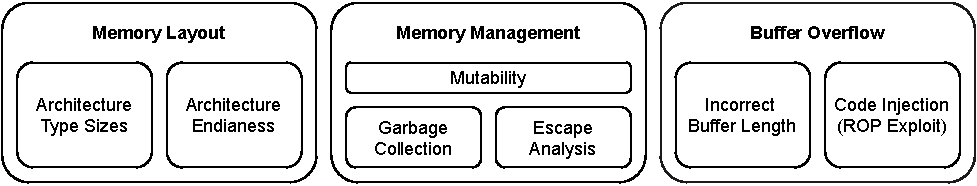
\includegraphics[width=\textwidth]{assets/figures/chapter3/outline3.pdf}
    \caption{Role of chapter 3 in the thesis outline}
    \label{fig:outline3}
\end{figure}



%% ---------------------------------------------------------------------------------------------------------------------

\section{Architecture-Dependent Types}\label{sec:unsafe-security-problems:architecture-dependent-types}

The first area of possible vulnerabilities is about types that have a different size or alignment on various
architectures.
A feature of Go is portability between different platforms~\cite{brimzhanova2019}.
The same source code can usually be compiled for many architectures without any changes in its behavior.
However, this is only true as long as the \unsafe{} \acrshort{API} is not used.
Since \unsafe{} code allows direct conversion between arbitrary types, there can be inconsistencies between the sizes
and alignments of structure fields on different architectures.
An example of this is shown in Listing~\ref{lst:architecture-dependent-types-cast}.
There are two structure types declared, \textit{PinkStruct} (Lines~1--4) and \textit{VioletStruct} (Lines~5--8), both of
which have two fields \textit{A} and \textit{B}.
While field \textit{B} has the same type (\textit{uint8}) in both types, field \textit{A} is of type \textit{int}
(Line~2) and \textit{int64} (Line~6), respectively.
An instance of \textit{PinkStruct} is created in Line~11, which is converted to \textit{VioletStruct} in Line~12.
This is only a valid operation if \textit{int} and \textit{int64} share the same size and alignment.

\begin{lstlisting}[language=Golang, label=lst:architecture-dependent-types-cast, caption=Incorrect cast between architecture-dependent types]
func main() {
    bytesResult := GetBytes()
    fmt.Printf("main: \%s\n", bytesResult) // expected (but failed) stdout is "abcdefgh
}

func GetBytes() []byte {
    reader := bufio.NewReader(strings.NewReader("abcdefgh"))
    s, _ := reader.ReadString('\n')
    out := StringToBytes(s)
    fmt.Printf("GetBytes: \%s\n", out) // expected stdout is "abcdefgh"
    return out
}
\end{lstlisting}

This is true for 64-bit platforms like \textit{amd64}.
If the code is executed on such an architecture, the conversion works fine and the field values in the resulting variable
\textit{violet} are as expected.
In contrast, if the code is run on an architecture where \textit{int} and \textit{int64} have different sizes or
alignments, the values of \textit{violet} are undefined.
This is the case, for example, on a 32-bit platform like \textit{i386}.
When the structure definitions are not placed directly next to each other but in separate files, packages, or even
modules, spotting the difference between the incompatible structs is much harder.
On top of that, the bug might never occur in testing but only on specific platforms that get used in production.
Possible consequences of a bug like this depend on how the resulting struct value is used in the remainder of the
program.
If data gets written to it, it changes invalid memory which can lead to a code injection vulnerability, and if it is
passed as output it can create an information leak vulnerability.

In addition to incompatible field sizes, there could also be a different byte order on some architecture.
In this case, using a direct cast using the \unsafe{} \acrshort{API} is unaware of possible changes of the byte order,
for example, incoming network data and variables stored in the memory could be represented as big and little endians and
cause a mismatch.
When such data is stored as the length of a slice, the number could be misinterpreted and, thus, a slice with a wrong
length could be created.
This in term can cause a buffer overflow vulnerability that can lead to code injection.

\begin{insight}
    Different type sizes and byte order on various architectures, used with direct conversions through
    \textit{unsafe.Pointer}, can cause invalid memory access such as buffer overflows.
\end{insight}


%% ---------------------------------------------------------------------------------------------------------------------

\section{Incorrect Slice and String Casts}\label{sec:unsafe-security-problems:slice-casts}

The second main area of danger with \unsafe{} usages is focused around the conversion of slices of different types, and
strings.
Listing~\ref{lst:string-to-bytes} shows a common \unsafe{} usage pattern that takes a string argument and converts it
into a slice of bytes without allocating additional memory.
This allows to access the raw bytes contained in the string in an efficient manner.

\begin{lstlisting}[language=Golang, label=lst:string-to-bytes, caption=Conversion from \textit{string} to \textit{[]byte} using \unsafe{}]
func StringToBytes(s string) []byte {
    strHeader := (*reflect.StringHeader)(unsafe.Pointer(&s))
    bytesHeader := reflect.SliceHeader{
        Data: strHeader.Data,
        Cap:  strHeader.Len,
        Len:  strHeader.Len,
    }
    return *(*[]byte)(unsafe.Pointer(&bytesHeader))
}
\end{lstlisting}

First, the string is converted into the \textit{reflect.StringHeader} representation in Line~2.
Then, a slice header is created as a composite literal and the reference to the underlying data array and length
information are copied from the string header (Lines~3--7).
The capacity is set to the same value as the length, as it would be in a slice that uses the full capacity.
Finally, the slice header is converted into an actual \textit{[]byte} slice which is returned (Line~8).

There are three non-obvious but potentially dangerous problems that come with this type of slice creation, which are
described in the following subsections.

%% ---------------------------------------------------------------------------------------------------------------------

\subsection{Implicit Immutability}\label{subsec:unsafe-security-problems:slice-casts:read-only}

The first problem is that the resulting slice is implicitly immutable, or read-only.
Regularly, slices in Go are mutable and strings are not.
As described in Section~\ref{sec:background:slices}, this is because the underlying string data array is usually located
on a read-only memory page.
If a developer writes code that changes parts of a string in-place, the compiler will not accept that code and, thus,
prevent the possible segmentation fault.

The slice returned by the \textit{StringToBytes} function in Listing~\ref{lst:string-to-bytes} is mutable.
Code that changes the resulting slice will be accepted by the compiler because it is not able to infer its connection to
a former string.
However, since the slice uses the same underlying data array as the original string used to do, the data is still
potentially located within read-only memory, and modifying it will crash the program.
It is only implicitly read-only, but the runtime is not aware of it.

While this first problem of the conversion pattern does not cause a direct security vulnerability, it underlines that
there are many consequences of using the \unsafe{} \acrshort{API} that are not obvious.
Although it is possible in theory to manually ensure that no usages of the \textit{StringToBytes} function modify the
slice it returns, in practice it is very hard to do so, especially if new developers join the project after some time
and start using the function without having all possible consequences in mind.

\begin{insight}
    Using in-place conversions using the \unsafe{} API can create fragile code with implicit rules that all developers
    working on the code need to follow to maintain correctness.
\end{insight}


%% ---------------------------------------------------------------------------------------------------------------------

\subsection{GC Race Use-After-Free}\label{subsec:unsafe-security-problems:slice-casts:gc-race}

The second problem with the conversion shown in Listing~\ref{lst:string-to-bytes} is a \textit{use-after-free} bug
caused by a race condition involving the garbage collector (\acrshort{GC}) used by the Go runtime.
As discussed in Section~\ref{subsec:background:memory:gc}, the \acrshort{GC} treats all pointer types and the special
\textit{Data} field of actual slices and strings as reference types.
Importantly though, it does not treat normal \textit{uintptr} values and \textit{Data} fields of artificially
constructed slice and string headers as references although they contain addresses.
This means that converting a \textit{uintptr} value to an \textit{unsafe.Pointer} value is an invalid and dangerous
operation.
If the \textit{GC} runs while the pointer has not been constructed, it does not mark the value at the address
stored in the \textit{uintptr} value as live and thus frees the memory.
Creating an \textit{unsafe.Pointer} from this address therefore creates a potentially dangling pointer, because it
points to memory that has been freed.
This is a \textit{use-after-free} bug.

Listing~\ref{lst:string-to-bytes} contains this bug.
The \textit{Data} field of the \textit{reflect.SliceHeader} structure created in Line~3 is of type \textit{uintptr}.
The header value is not derived by cast from a real slice.
Therefore, it does not benefit from the special case built into the Go runtime, which treats \textit{uintptr} references
that are part of slices and strings as references.
Specifically, the problem is that the slice header has been constructed as a composite literal.
Therefore, after Line~7 the \textit{bytesHeader} variable becomes a plain \textit{uintptr} value, and the
original string \textit{s} is not used any longer.
However, at this point there is no real slice created yet as this happens not earlier than in Line~8.
The underlying data array of the string \textit{s} is therefore not a live value as far as the \acrshort{GC} is
concerned.
If the \acrshort{GC} runs at this time, the underlying data array used in the slice is already collected when the
resulting slice is created.
This is possible because the \acrshort{GC} runs concurrently to the application logic and can trigger at any time.
If the Go program has several threads that all contribute to the heap usage, this is even more severe.

\begin{figure}[!t]
    \vspace{2mm}
    \centering
    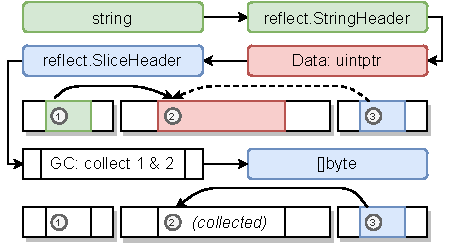
\includegraphics[width=0.4\textwidth]{gfx/figures/gcrace-vuln.pdf}
    %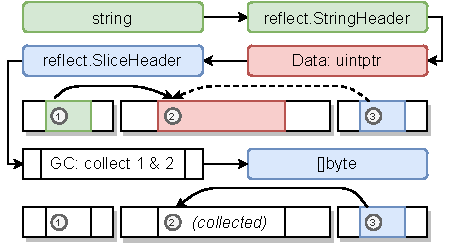
\includegraphics[width=0.48\textwidth]{gfx/figures/gcrace-vuln.pdf}
    \caption{GC race and escape analysis flaw}
    \label{fig:gcrace-vuln}
    \vspace{-8pt}
\end{figure}


Figure~\ref{fig:gcrace-vuln} illustrates the vulnerability.
The green boxes show the original string value and its header (Line~2 in Listing~\ref{lst:string-to-bytes}), which is
represented at position 1 in the memory schema.
The reference to the underlying data of the string and resulting slice (Line~4) is shown in red at memory position 2.
Then, the slice header is created (Lines~3--7), which is colored blue and located at position 3 in the memory.
References indicated by arrows are strong if the arrow is continuous, like the reference the string header has, and
weak if the arrow is dashed, like the new slice header has.
Then, after the \textit{GC} runs, there is only the resulting bytes slice left, which is also shown in blue.
It now has a strong reference to the underlying data array (at position 2), but since the \acrshort{GC} has already run
while there was only a weak reference to it, the data has been collected.
The resulting bytes slice (Line~8) is now a dangling pointer into the former string data in memory, and the
\textit{use-after-free} bug is complete.

If the bytes slice is modified, arbitrary memory is changed.
This can allow an attacker to tamper with application data, or possibly change stored return addresses on the stack,
therefore achieving a code injection vulnerability.


%% ---------------------------------------------------------------------------------------------------------------------

\subsection{Escape Analysis Use-After-Free}\label{subsec:unsafe-security-problems:slice-casts:escape-analysis}

The third problem that comes with the incorrect construction of a new slice shown in Listing~\ref{lst:string-to-bytes}
is that the Go compiler's escape analysis (\acrshort{EA}) algorithm fails.
For a similar reason to the \acrshort{GC}, it misses the connection between the string parameter and the slice return
value.
Listing~\ref{lst:escape-analysis-flaw} shows a proof of concept of this problem.

\begin{lstlisting}[float=tp, language=Golang, label=lst:escape-analysis-flaw, caption=Escape analysis flaw proof of concept]
func main() {
    bytesResult := GetBytes()
    // expected stdout is "abcdefgh"
    // actual output is random invalid data
    fmt.Printf("main: %s\n", bytesResult)
}

func GetBytes() []byte {
    reader := bufio.NewReader(strings.NewReader("abcdefgh"))
    s, _ := reader.ReadString('\n')
    out := StringToBytes(s)
    // expected stdout is "abcdefgh"
    // actual output is "abcdefgh"
    fmt.Printf("GetBytes: %s\n", out)
    return out
}
\end{lstlisting}

In the function \textit{GetBytes}, a string variable \textit{s} is created by reading a string through a buffered
reader (Lines~9--10).
It is necessary to use the reader instead of a string literal, because with a literal the effects of the vulnerability
would not be visible.
This is however no restriction to the generality of this proof of concept.
Creating the string from a reader is similar to accepting dynamic user input.
Next, the string is converted to a byte slice using the insecure \textit{StringToBytes} function
(Listing~\ref{lst:string-to-bytes}) in Line~11.
Printing the resulting slice in Line~14 yields the expected output equal to the original string, which is
\textit{abcdefgh}.
Finally, the slice is returned to the caller function, which in this case is the \textit{main} function in Line~2.
The slice is printed again in the \textit{main} function in Line~5, and while the expected output would be identical,
this time invalid, random data is printed.

The reason for this is that when the Go \acrshort{EA} algorithm determines where to allocate the string \textit{s} in
the \textit{GetBytes} function, it detects that \textit{s} is passed to the \textit{StringToBytes} function and
therefore transitively analyzes that function.
Within the function, \textit{s} is used in a cast to the \textit{strHeader} variable in Line~2 of
Listing~\ref{lst:string-to-bytes}.
After that, \textit{strHeader} is used to construct the \textit{bytesHeader} variable, but at this point there are no
further references to the underlying data array of \textit{s}.
The reason for this is that both \textit{s} and \textit{strHeader} are not used further in the function.
Similarly to the \acrshort{GC} mark algorithm, the \textit{Data uintptr} field would only be treated as a reference with
respect to escape analysis if the slice header had been created by cast from an actual slice.
Therefore, the \acrshort{EA} determines that \textit{s} does not escape in \textit{StringToBytes}, and since it is not
used any longer in \textit{GetBytes}, it does not escape at all and is placed on the stack of the \textit{GetBytes}
function.
The \textit{EA} algorithm fails to detect that there is a reference to the string \textit{s} in the \textit{out}
variable, which obviously escapes as it is returned.

Printing the \textit{out} slice in Line~15 works because the stack of the \textit{GetBytes} function still exists at
this point.
However, when the function returns, the stack frame is removed, and \textit{bytesResult} in Line~2 becomes a dangling
pointer into the former stack of \textit{GetBytes}.
This is a \textit{use-after-free} bug because that memory can and probably will be reused at that point.
The print statement in Line~5 outputs invalid data for this reason.
If the \textit{main} function would modify the contents of the \textit{bytesResult} slice, it would change arbitrary
memory, with possible consequences such as information leaks or code injection.

\begin{insight}
    Creating slice or string headers from scratch is an invalid and dangerous operation, because the Go \acrshort{GC}
    and \acrshort{EA} do not recognize the reference to the underlying array in memory.
    This causes \textit{use-after-free} bugs for multiple reasons, and can result in access to arbitrary memory and code
    injection for an attacker.
\end{insight}


%% ---------------------------------------------------------------------------------------------------------------------

\section{Buffer Overflow Vulnerabilities}\label{sec:unsafe-security-problems:buffer-overflow}

The third main area of possible vulnerabilities in the context of the \unsafe{} \acrshort{API} are buffer overflows.
In the following subsections, different ways of creating buffer overflows are discussed, and a concrete example of
using a vulnerability with return-oriented programming (\acrshort{ROP}) is given.


%% ---------------------------------------------------------------------------------------------------------------------

\subsection{Incompatible Types}\label{subsec:unsafe-security-problems:slice-casts:incompatible-types}

Converting slices to strings and vice versa can be done simply by casting them, however this will cause the Go runtime
to allocate a new slice or string for the resulting value.
To improve efficiency by reusing the underlying data and only reinterpret it as a new type, it is possible to use the
\unsafe{} \acrshort{API} for an in-place cast.
Since the fields in the header structures shown in Listing~\ref{lst:reflect-header-types} in
Section~\ref{sec:background:slices} are different in the presence of the \textit{Cap} field, this is however only valid
for conversions from slices to strings.
In that case, the resulting string header, which shares the same location in memory with the original slice header, will
reuse the reference to the underlying data array as well as the length, and since the string header structure does not
contain any more fields the capacity information will be unused although it remains in adjacent memory.

In contrast, when converting a string to a slice directly, the source header structure is too short.
The resulting slice header will use correct values for its data reference and length, but the capacity field will
contain whatever is located in memory directly after the original string header.
This is shown in Listing~\ref{lst:unsafe-string-to-bytes-direct}, which is taken from the \textit{k8s.io/apiserver}
package that is part of the \textit{Kubernetes} project\footnote{\url{https://github.com/kubernetes/apiserver}}.

% k8s.io/apiserver/pkg/authentication/token/cache/cached\_token\_authenticator.go:235

\begin{lstlisting}[language=Golang, label=lst:unsafe-string-to-bytes-direct, caption=Incorrect direct cast between string and slice]
// toBytes performs unholy acts to avoid allocations
func toBytes(s string) []byte {
    return *(*[]byte)(unsafe.Pointer(&s))
}
\end{lstlisting}

The resulting slice (Line~3) is dangerous to use, because it contains random data in its capacity field.
Operations that read from a slice, like using it in a loop to iterate over its contents, mostly only use the data
reference and length.
However, any action on the slice that uses the capacity, like taking subslices from it or appending data, is undefined
and can therefore become a security vulnerability.
A slice with a capacity that is greater than the actual allocated memory can be used to read and write adjacent memory
by increasing its length until it reaches outside its valid bounds.
Thus, an attacker can control invalid memory, leading to possible code injection or information leak.

\begin{insight}
    Operations that seem to be valid in two directions, and in fact look symmetric both ways, can be incorrect in one of
    the directions.
    Using the \unsafe{} \acrshort{API}, this can create an exploitable buffer overflow vulnerability.
\end{insight}


%% ---------------------------------------------------------------------------------------------------------------------

\subsection{Incorrect Length Information}\label{subsec:unsafe-security-problems:slice-casts:incorrect-length}

Buffer overflows can also be caused by creating a new slice that has an incorrect length with respect to its underlying
data array.
This can happen quickly if the length information is calculated dynamically, especially if user-supplied input data is
used to deduce the resulting value.
An example of such a bug is shown in Listing~\ref{lst:go-fuse-bug}.
It is taken from the \textit{hanwen/go-fuse} library\footnote{\url{https://github.com/hanwen/go-fuse}}, a Go
implementation of the server specification used for the userspace file system (\acrshort{FUSE}) available for
Linux\footnote{\url{https://www.kernel.org/doc/html/latest/filesystems/fuse.html}}.
A patch for this bug has already been submitted to the authors.

% github.com/hanwen/go-fuse fuse/opcode.go:299

\begin{lstlisting}[language=Golang, label=lst:go-fuse-bug, caption=Incorrect slice length bug in the \textit{hanwen/go-fuse} library]
func doBatchForget(server *Server, req *request) {
    in := (*_BatchForgetIn)(req.inData)
    wantBytes := uintptr(in.Count) * unsafe.Sizeof(_ForgetOne{})

    if uintptr(len(req.arg)) < wantBytes {
        // We have no return value to complain, so log an error.
        log.Printf("Too few bytes for batch forget.",
                   len(req.arg), wantBytes, in.Count)
    }

    h := &reflect.SliceHeader{
        Data: uintptr(unsafe.Pointer(&req.arg[0])),
        Len:  int(in.Count),
        Cap:  int(in.Count),
    }
    forgets := *(*[]_ForgetOne)(unsafe.Pointer(h))
    // ...
}
\end{lstlisting}

\acrshort{FUSE} uses a client / server architecture where file system implementations present a server that handles
requests from a specific kernel module.
The listing shows a part of the \textit{doBatchForget} function, which is used to clear files, identified by their inode
number, from a cache that the file system might have.
In the design of \textit{go-fuse}, incoming data from the \textit{/dev/fuse} node is passed to handler functions as byte
slices (\textit{req.inData} and \textit{req.arg} in Lines~2 and~5) containing the raw, serialized request.
The handler function then casts the data into a suitable structure to access individual fields.
In this case, the request is converted into an instance of the \textit{\_BatchForgetIn} type (Line~2), which provides
access to the number of inodes to forget in the batch request through the \textit{in.Count} field (Line~3).
The individual forget messages in serialized and concatenated form are available through the \textit{req.arg} array, so
to access them a new slice is created by defining its slice header from scratch (Lines~11--15).
The created slice uses the incoming request data containing the forget messages (\textit{req.arg}, Line~12) as its
underlying data array, and the number of messages (\textit{in.Count}) both as length and capacity (Lines~13 and~14).

Since the \textit{in.Count} field is supplied as part of the request sent to the library, it can be controlled by an
attacker if they manage to conduct a man-in-the-middle attack and change the request to be a malicious one.
If the length is greater than the available number of data bytes, the resulting \textit{forgets} slice (Line~16) will
access additional data after the end of the actual \textit{batch forgets} request.
Depending of the concrete operation to prune inodes from a local cache, this could have severe consequences with respect
to security.
To prevent this from happening, the authors intended to check the length of the available data in Line~5, and if there
are too few bytes for the alleged number of individual requests, the method should not proceed.
However, as the listing shows there is no actual code to stop further execution of the method, instead there is only a
log message noting that there was a malformed request with too few bytes available (Lines~7--8).

A proof-of-concept implementation\footnote{\url{https://github.com/jlauinger/go-unsafepointer-poc}} of a potential
exploit showed that the method actually accesses invalid memory data located after the request data.
Depending on the code that calls this function, an attacker can use this to read or write this memory, again possibly
enabling arbitrary code injection or information leak exploits.
In this case, a simple \textit{return} statement after Line~8 would have prevented this bug.

\begin{insight}
    In Go code that uses the \unsafe{} \acrshort{API}, developers who fail to implement proper bounds checking can
    quickly cause very serious security vulnerabilities.
    Code then has to be written and audited as carefully as traditional, non-memory-safe C code.
\end{insight}


%% ---------------------------------------------------------------------------------------------------------------------

\subsection{Code Injection using ROP}\label{subsec:unsafe-security-problems:buffer-overflow:code-flow-redirection}

This section shows practical evidence that buffer overflows as described in the previous sections can actually cause an
attacker to achieve code injection.
This is done by outlining a proof-of-concept exploit using return-oriented programming (\acrshort{ROP}), the source code
of which is available on \github{}\footnote{\url{https://github.com/jlauinger/go-unsafepointer-poc}}.

Listing~\ref{lst:buffer-overflow} shows a short example function that contains a buffer overflow.
In Line~4, a byte slice with a length of 512 bytes is initialized.
Then, its slice header is obtained in Line~5 and used to change the underlying data array of the slice (Line~6).
After the switch, the slice is backed up by a much shorter byte buffer of eight bytes (initialized in Line~2).

\begin{lstlisting}[language=Golang, label=lst:buffer-overflow, caption=Buffer overflow leading to code flow redirection]
func main() {
    harmlessData := [8]byte{'A', 'A', 'A', 'A', 'A', 'A', 'A', 'A'}

    confusedSlice := make([]byte, 512)
    sliceHeader := (*reflect.SliceHeader)(unsafe.Pointer(&confusedSlice))
    sliceHeader.Data = uintptr(unsafe.Pointer(&(harmlessData[0])))

    _, _ = bufio.NewReader(os.Stdin).Read(confusedSlice)
}
\end{lstlisting}


Then, a reader is used to read input data into this malicious slice in Line~8.
Since it has a length of 512 bytes, the function reads up to this many bytes, however because the actual data array used
by the slice is much shorter, this will overflow into the memory behind the data array.
In this case, the \textit{harmlessData} array is created on the stack of the function, which means it is vulnerable to
stack-based buffer overflow exploits as described in Section~\ref{subsec:background:exploit-techniques:buffer-overflow}.
An attacker can use this vulnerability to redirect the code flow by carefully crafting the input data such that the
saved return instruction pointer on the stack is overwritten with the address of a function of the attacker's choice.

As described in Chapter~\ref{ch:background}, \acrshort{DEP} prevents directly putting exploit code on the stack, but
since the Go compiler uses static linking, \acrshort{ASLR} is not much of a concern.
Using \acrshort{ROP}, it is possible to use gadgets with machine instructions that are part of the Go standard library,
which is linked into the binary of all Go applications.
A strategy to exploit a buffer overflow to achieve code injection is to use the \textit{mprotect} and \textit{read}
system calls.
A system call, or syscall, is a function provided by the operating system, which can be executed using the
\textit{syscall} machine instruction.
The processor registers control which syscall gets executed and which parameters it receives.
Therefore, an attacker needs \acrshort{ROP} gadgets to control the contents of the registers, as well as to trigger
the syscall.
There are several alternative gadgets for this available in the Go standard library.

Using the \textit{mprotect} call, the attacker can set a memory area of their choice to have both writable and
executable flags, for example, the heap area.
Then, using the \textit{read} call, they can store data in that memory section, which is usually an exploit payload
spawning a shell to receive further arbitrary commands.
The payload is provided as part of the input string created by the attacker.
Finally, by using the address of the code area just like an address of another \acrshort{ROP} gadget the attacker can
make the processor jump to the payload code.
Because in contrast to the stack the code is located on an executable page, the \acrshort{CPU} executes it and the code
injection attack succeeds.
This clearly demonstrates the severeness of buffer overflows introduced through misuses of the \unsafe{} \acrshort{API}
in Go programs with concrete evidence on how to create a successful exploit.

\begin{insight}
    Once a Go program contains a buffer overflow vulnerability, established and well-researched exploit techniques like
    \acrshort{ROP} can be used just as in traditional languages like C to achieve code injection.
\end{insight}


%% ---------------------------------------------------------------------------------------------------------------------

\section{Summary}\label{sec:unsafe-security-problems:summary}

This chapter presented multiple different ways of misusing the \unsafe{} \acrshort{API} in Go applications.
Almost all of them can be used, in one way or another, to effectively inject and execute arbitrary code, or read and
modify protected data within the process memory.

Many of the dangers are correlated with slices and strings, and especially their internal structure that is accessible
through their header structures.
This is not surprising since slices are a close equivalent to buffers in other languages, which means they are often
concerned with user-supplied data, and inherently carry the danger of missing proper bounds checking.

More details and proof-of-concept exploit code for the vulnerabilities presented in this Chapter are available in a
dedicated repository on \github{}\footnote{\url{https://github.com/jlauinger/go-unsafepointer-poc}}.
